

\chapter{Étude de la structure d'un flot de liens}

L'étude de la structure des réseaux est un sujet qui est étudié depuis assez longtemps \REF.
Ces études ont, dans un premier temps, permis de trouver comment caractériser une structure puis, dans un second temps, de proposer des méthodes de détections de ces structures.
La littérature sur l'étude des flots de liens est encore récente et il n'existe que peu d'études \REF\ sur les spécificités des structures dans les flots de liens.

Nous nous intéressons à une archive de courriels publiquement disponibles\footnote{\url{https://lists.debian.org/debian-user/}}.
L'étude de fil de discussions a déjà étudié dans le passé~\cite{Dorat2007} mais cela a été fait en utilisant des méthodes statiquement.
Cette archives l'ensemble des courriels échangés par différent utilisateurs lors de l'utilisation de debian.
Typiquement, une personne ayant un problème lors de l'installation envoie un courriel à la liste afin de demander de l'aide.
Toutes personnes inscrites sur la liste reçoit cette demande et peut y répondre.
Ces données se transposent facilement sous forme de flot de liens car une personne est un n\oe uds et chaque courriel entre deux personnes donne lieu à un lien dans le flot à l'instant où le courriel a été envoyé.
Le message initiant la conversation est ignoré pour éviter les boucles.
L'avantage de ces données de communications est que nous connaissons la discussion dans laquelle a lieu chaque message.
Une discussion est un ensemble de courriels dont tout les messages répondent à un message précédant excepté pour le premier qui a initié la discussion et que nous appelons $racine$.
Ainsi, nous étudions la structure des discussions dans le flot liens représentant les courriels envoyés sur la liste.

Utiliser le formalisme de flot de liens est particulièrement intéressant car cette lite de diffusion existe depuis 1994.
L'aspect temporelle des discussion est donc important.



\section{Prétraitement sur le jeu de données}
Bien que disponible, ce jeu de données nécessite un ensemble de traitement avant de pouvoir exploiter les 724985 courriels que contenait l'archive en janvier 2015.
Tout d'abords, les données ne sont pas sous la forme d'un flot de liens avec la structure des conversations.
Les données sont accessibles via le site internet.
Pour avoir ces informations sous la forme d'un flots de liens, un script d'extraction a été développé \com{URL}.
Lors de l'extraction, 2269 courriels n'ont pas pu être pris en compte car certaines informations étaient manquantes ou mal formées.

Une fois les informations récupérées, il est nécessaire de vérifier leurs cohérences.
Pour chaque courriel, sont connus d'envoie, l'auteur, le destinataire, le courriel auquel il répond et la discussion dans laquelle il apparait.

Un message peut être filtré pour différentes raisons: le courriel apparait avant le message auquel il est censé répondre, le message auquel il réponds n'est pas présent dans l'archive, l'auteur et le destinataire sont la même personne\footnote{Ce cas est relativement rare.}.
Il s'agit de vérifications simple auquel il faut ajouter les vérification de la cohérence de la structure de discussions.
Ainsi, une discussion est retirée du jeu de donnée si il manque la racine, un de ces messages a été retiré précédemment ou si la discussion a débuté trop récemment ou si elle dure trop longtemps.
Les deux dernières conditions permettent d'éviter un biais envers les conversations incomplètes car trop longues ou trop récentes.
La limite pour considérer une discussion trop récente ou trop longue a été fixé à 2 ans en observant la distribution de durées des discussions, voir la figure~\ref{fig:dists_discussion}.

Une fois tout ces messages filtrés, nous obtenons un flot de liens avec 554233 liens entre 34648 personnes pendant presque 19 ans et 116999 discussions.
Mis à part les courriels de début de discussions, ce sont 53753 courriels qui ont été filtrés soit environ $7\%$.

\inline{Parler de la transformation données vers formalisme flot}
\section{Caractéristiques basiques des discussions}

Les caractéristiques les plus basiques des discussions sont le nombre de courriels, le nombre de personnes, le nombre de paires de personnes distincte en interaction direct et leur durée.
Sur la figure~\ref{fig:dists_discussion} sont présentes les distributions cumulatives inverses de ces notions et on remarque qu'elles sont hétérogènes.

\begin{figure}
\centering
	\includegraphics[angle=-90, width=0.49\linewidth]{img/mailing/sizes-ccdf.eps}
	\includegraphics[angle=-90, width=0.49\linewidth]{img/mailing/durations-ccdf.eps}\\
	\includegraphics[angle=-90, width=0.49\linewidth]{img/mailing/authors-ccdf.eps}
	\includegraphics[angle=-90, width=0.49\linewidth]{img/mailing/authorpairs-ccdf.eps}
	
	\caption{Distribution cumulative inverse de différentes caractéristiques pour les données brutes (ligne pleine) et filtrées (ligne pointillé). En haut à gauche: nombre de courriels dans une discussion; en haut à droite: durée d'une discussion; en bas à gauche: nombre de personnes dans une discussion; en bas à droite: nombre de paires d'auteurs distinct dans une .}
	\label{fig:dists_discussion}
\end{figure}

La distribution des durées des discussions, mets en avant que la majorité des discussions dure environ une journée (100000 secondes équivaux à moins de 28 heures).
Par ailleurs, on remarque qu'il n'existe que quelques discussions durant plus d'un an.
C'est pourquoi, la limite sur la durée a été fixée à 2 ans.
Enfin, on remarque que les données filtrées ne diffèrent pas qualitativement des données brutes.

Ces premières observations sont nécessaires mais pas suffisante pour comprendre les caractéristiques d'une discussion.
Nous avons également étudié la corrélation de ces différentes notions et une partie d'entre elles sont présentées sur la figure~\ref{fig:corr_discussion}.


\begin{figure}
	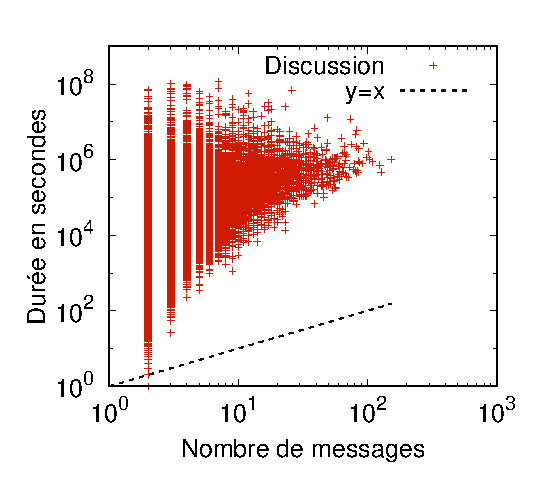
\includegraphics[angle=-90, width=0.49\linewidth]{img/mailing/sizes-durations-corr.eps}
	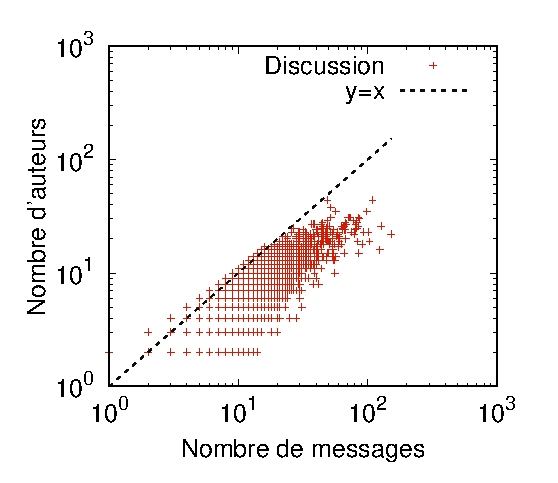
\includegraphics[angle=-90, width=0.49\linewidth]{img/mailing/sizes-authors-corr.eps}
	\caption{Gauche: Corrélations entre le nombre de courriels et la durée d'une discussion. Droite: Corrélation entre le nombre de courriels et le nombre d'auteurs dans une discussion.}
	\label{fig:corr_discussion}
\end{figure}

La corrélation entre la durée et le nombre de courriels, figure de gauche, mets en évidence que plus une discussion est grande en nombre de courriels plus elle dure longtemps ce qui est attendu.
Par contre, on observe également que les petites discussions ont des durées très variables. 
Sur la figure de droite présentant la corrélation entre le nombre de courriels et d'auteurs, on observe également un fait attendu~~\cite{Dorat2007} qui est qu'il y a plus de courriels que d'auteurs. Ainsi lors d'une discussion, c'est un petit nombre de personnes qui partagent beaucoup de messages. 

Enfin, il est intéressant d'observer la dynamique des échanges entre deux personnes.
Soit $\tau(u,v) = (t_{i+1}-t_i)_{i=0..k+1}$ la séquence des temps inter-contacts d'une pair de n\oe uds $u$ et $v$ dans $V$\note{$t_0=\alpha$ et $t_k+1=\omega$}.
Il s'agit du temps écoulé avant que deux personnes se contactent à nouveau.
Sur la figure~\ref{fig:ict_discussion} est représentée la distribution cumulative inverse du temps inter-contacts. 
On remarque que $21\%$ des temps inter-contacts est inférieurs à 30 jours.
Ce chiffre bien que relativement faible est tout de même important car il s'agit d'un fil de discussions ouvert où tout le monde peut participer. 
En particuliers, une personne peut envoyer une demande d'aide à un moment donner et ne plus jamais participer.
\begin{figure}
	\centering
	\includegraphics[width=0.49\linewidth]{img/mailing/ict-ccdf.eps}
	\caption{Distribution des temps inter-contacts dans le fil de discussions.}
	\label{fig:ict_discussion}
\end{figure}

\section{\'Etude des discussions en tant que sous-flots}
\subsection{Applications de la densité aux discussions}

Jusqu'à maintenant aucune notion intrinsèquement liées aux flot de liens n'a été utilisée pour caractériser les discussion et leur répartition dans le flot de liens.
Le but est d'évaluer si cette structure de flot peut se rapprocher d'une structure communautaire.
Comme dit précédemment, les communautés sont souvent définies comme étant des structure devant être densément connectées.
C'est pourquoi nous nous attachons à étudier la densité des discussions.

Comme ces données se modélisent par un flot de liens ou chaque lien n'a pas de durée, nous étudions la $\Delta$-densité pour différentes valeurs de $\Delta$.
Tout d'abord sur la figure~\ref{fig:dens_fil_discusion} est représenté la $\Delta$-densité globale de tout le flot de liens.
En couvrant un spectre aussi large de $\Delta$, on observe que la $\Delta$-densité est croissante avec $\Delta$ mais surtout on observe bien la convergence de $\Delta$-densité vers la densité du graphe agrégé lorsque $\Delta$ est proche de $\omega - \alpha$.
\inline{Ajout bar horizontal de la densité statique.}

\begin{figure}
	\centering
	\includegraphics[width=0.48\linewidth]{img/mailing/global_linlin.eps}
	\caption{Évolution de la $\Delta$-densité du flot de liens pour $\Delta$ de $1$ seconde à $20$ ans.}
	\label{fig:dens_fil_discusion}
\end{figure}

La $\Delta$-densité du flot liens, cependant, n'apporte que peu d'informations en elle-même.
Elle est surtout utile pour comparer les valeurs de $\Delta$-densité des sous-flots que sont les discussions.
Ainsi sur la figure~\ref{fig:intra_dens_discussion} est présentée la distribution cumulative inverse de la $\Delta$-densité des discussions pour différentes valeurs de $\Delta$.
On remarque que les différentes valeurs de $\Delta$ ne semblent pas influencer qualitativement la distribution de $\Delta$-densité.
Cette courbe mets surtout en évidence que les discussions sont des structures beaucoup plus denses que le flot.
En effet, la densité médiane des discussions est, selon la valeur de $\Delta$, entre $2.69 \times 10^{-4}$ et $0.28$ alors que le flot a une densité entre $1.05  \times 10^{-10}$ et $3.42 \times 10^{-5}$.
La $\Delta$-densité des discussions est donc en moyenne $10^{5}$ fois plus élevé que celle du flot.
Bien que notable, ce fait est attendu notamment car le flot dure beaucoup plus longtemps et concerne beaucoup plus de n\oe uds que les discussions.
\begin{figure}
\centering
%\subfloat[Inverse cumulative distribution of intra-threads density.]{
	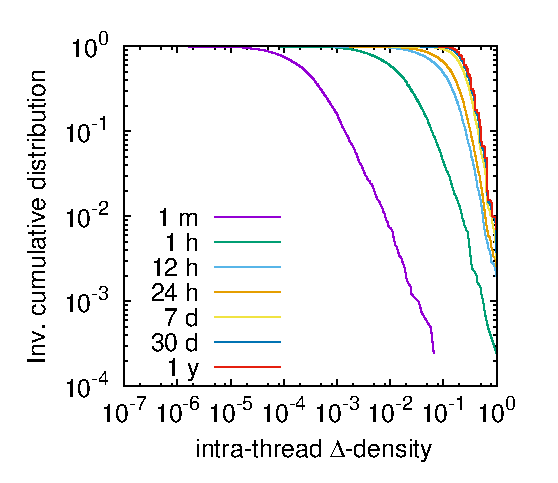
\includegraphics[width=0.48\linewidth]{img/mailing/delta.eps}
%}

\caption{Distribution cumulative inverse de la $\Delta$-densité des discussions pour différentes valeurs de $\Delta$s.}
\label{fig:intra_dens_discussion}
\end{figure}

Afin d'aller plus loin dans l'étude de cette structure, il faut revenir à une définition plus précise de ce qu'est une bonne communauté.
En soit, une valeur de densité n'est pas une preuve pour définir une structure comme communautaire.
En effet, une discussion ayant une densité de $0.8$ peut  ne pas être une communauté tant dis qu'une autre ayant une densité proche de zéro peut être une communauté.
Il faut définir un point de comparaison pour effectivement affirmer qu'une structure est particulièrement dense.
La prise en compte de la densité globale est un début mais n'est pas suffisante.
\note{Faire SNAM sur les threads}

Une autre définition d'une communauté est qu'une communauté devrait être plus densément connecté à l'intérieur qu'avec les autres communautés adjacentes.
Pour un graphe $G=(V,E)$ et une communauté $C_i$ de la partition $C = \{C_j\}_{j_1..k}$ de $V$ en $k$ communautés, cela se traduit par le calcul de la densité entre les communautés, $\delta^{inter}(C_i)$ :

\begin{equation}
	\delta^{inter}(C_i) = \frac{1}{|C|-1}\sum_{j, i\ne j}\frac{|\{(u,v)\in E\mbox{ s.t. }u\in C_i\mbox{ and }v\in C_j\}|}{|C_i|\cdot |C_j|}
\end{equation}

où $\delta(G_{ij})$ est la densité du graphe constitué des n\oe uds des communautés $i$ et $j$ et liens de $G$ entre ces deux communautés.
Il s'agit tout simplement de la probabilité qu'il y un lien existe entre les n\oe uds des deux communautés.
Encore une fois, cette notion n'a pas de sens direct dans le formalisme de flot de lien et il est nécessaire de l'adapter.
Pour ce faire, nous définissons le sous-flot inter-discussion entre les discussion $D_i$ et $D_j$ de la manière suivante:  $L_{ij} = (T_{ij}, V_{ij}, E_{ij})$, avec $T_{ij} = [$min($\alpha_i,\alpha_j$), max($\omega_i, \omega_j$)$]$, $V_{ij} = V_i\cup V_j$ et $E_{ij} = \{(t,u,v): t\in T_{ij}, u,v\in V_{ij}, (t,u,v)\in E\setminus D_i\cup D_j\}$\note{C'est pas vraiment ça ...}.
\note{Faire un dessin de cette situation?}
La $\Delta$-densité inter discussions entre $D_i$ et $D_j$ est alors la $\Delta$-densité du sous-flot $L_{ij}$.
Afin d'obtenir la $\Delta$-densité inter discussions entre $D_i$ et tout les autres discussions, nous utilisons la moyenne des densité inter discussion entre $D_i$ et les autres discussions, soit:

\begin{equation}
	\delta^{inter}_{\Delta}(D_i) = \frac{1}{|C|-1}\sum_{j,i\ne j} \delta_{\Delta}(L_{ij}).
\end{equation}

La distribution cumulative inverse de la $\Delta$-densité inter discussions est sur la figure~\ref{fig:inter_dens_discussion} pour différentes valeurs de $\Delta$.
Bien que similaire, le comportement qualitatif de la $\Delta$-densité inter discussions diffère de la $\Delta$-densité des discussions.
La $\Delta$-densité inter discussions croit également en fonction de $\Delta$ mais il y a toujours une différence notable entre $\Delta= 1\  mois$ et $\Delta= 1\ ann\acute{e}e$ ce qui n'est pas le cas pour la $\Delta$-densité.
Cette différence est normal car lors du calcul de $\Delta$-densité le nombre de liens considérés est fixe peut import $\Delta$ alors qu'il croit avec $\Delta$ lors du calcul de $\Delta$-densité inter discussions.
\note{Peut etre aussi parce que $L_{ij}$ dure plus longtemps}
\begin{figure}
\centering
%\subfloat[Inverse cumulative distribution of inter-threads density.]{
	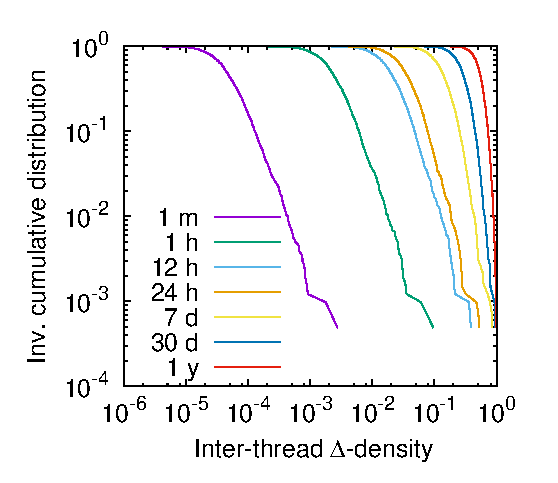
\includegraphics[width=0.48\linewidth]{img/mailing/inter_delta.eps}
%}
\caption{Distribution cumulative inverse de la $\Delta$-densité inter discussions pour différentes valeurs de $\Delta$s.}
\label{fig:inter_dens_discussion}
\end{figure}


Afin de comparer plus aisément $\Delta$-densité et $\Delta$-densité inter discussions, la corrélation entre ces deux mesures est présentée sur la figure~\ref{fig:corel_inter_discussion} pour différentes valeurs de $\Delta$.
On remarque que les discussions sont effectivement plus dense intérieurement qu'avec les autres discussions.
La différence est de plusieurs ordres de grandeur lorsque $\Delta$ est petit et elle diminue lorsque $\Delta$ croit.
Pour $\Delta=20\ ans$ sur la figure~\ref{fig:corel_inter_discussion_20}, la différence n'est plus visible car à cette échelle de temps, l'ancrage temporel des discussions n'est plus décisif.
Pourtant, on remarque que même pour $\Delta=1\ an$, la différence reste notable.
 

\begin{figure}[!h]
\centering
\subfloat[$\Delta= $1 minute]{
	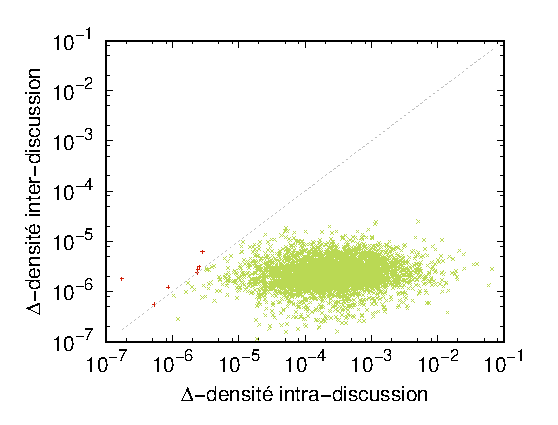
\includegraphics[width=0.48\linewidth]{img/mailing/DensityCurve/120/mean.eps}
}
\subfloat[$\Delta= $1 jour]{
	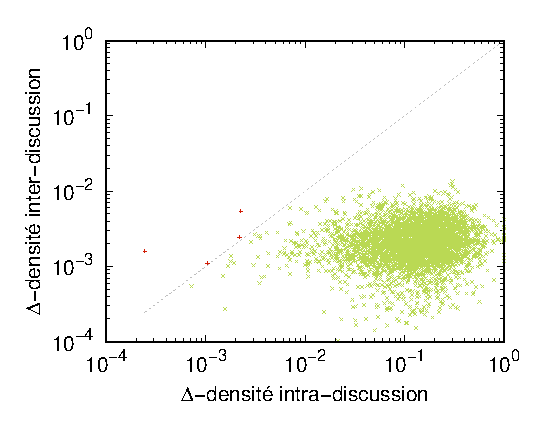
\includegraphics[width=0.48\linewidth]{img/mailing/DensityCurve/172800/mean.eps}
}

\subfloat[$\Delta= $1 an]{
	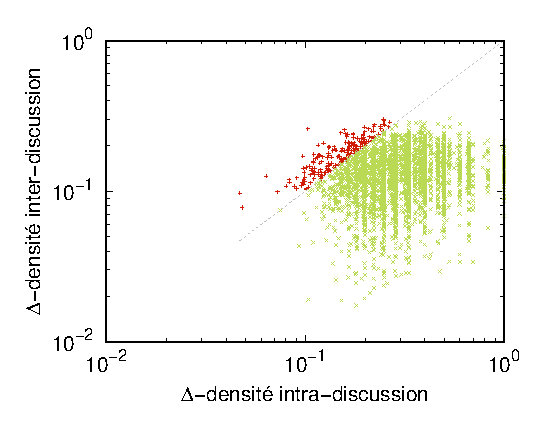
\includegraphics[width=0.48\linewidth]{img/mailing/DensityCurve/63072000/mean.eps}
}
\subfloat[$\Delta= $20 ans]{\label{fig:corel_inter_discussion_20}
	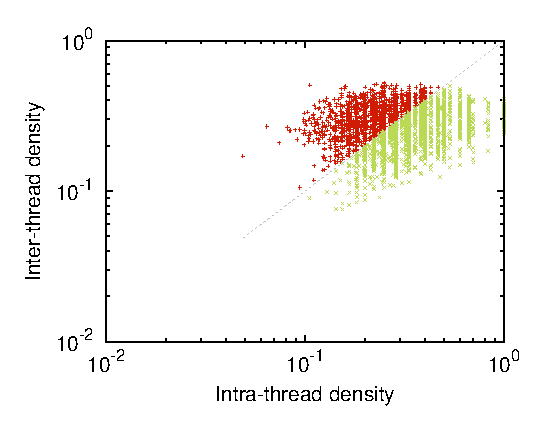
\includegraphics[width=0.48\linewidth]{img/mailing/DensityCurve/1261440000/mean.eps}
}
\caption{Corrélations entre $\Delta$-densité et $\Delta$-densité inter discussions pour différentes valeurs de $Delta$. Une discussion est en vert (resp. rouge) si elle a une $\Delta$-densité plus (resp. moins) élevée que sa $\Delta$-densité inter discussions.}
\label{fig:corel_inter_discussion}
\end{figure}

\subsection{Répartitions des discussions temporellement et structurellement}

Nous avons étudié la densité des discussions et entre les discussions mais il est également intéressant d'observer comment ces discussions sont réparties topologiquement et temporellement.
Pour étudier la répartition des discussions dans le temps, nous construisons un graphe $X=(V_X,E_X)$ d'intervalle\REF représentant le chevauchement temporel.
Chaque discussion du flot devient un n\oe uds de $V_X$ et le lien $(i,j)$ existe dans $E_X$ si les discussions $D_i$ et $D_j$ correspondantes ont eu lieu au même instant, \emph{i.e.} $[\alpha_i, \omega_i] \cap [\alpha_j, \omega_j] \neq \emptyset$.
De manière similaire, nous définissons le graphe de chevauchement topologique $Y=(V_Y,E_Y)$.
Les n\oe uds de se graphe représente encore une fois les discussions du flot et un lien existe entre discussion si au moins une personne participe aux deux discussions, \emph{i.e.} $V(D_i) \cap V(D_j) \neq \emptyset$.

Ces deux graphes sont constitués de 116999 n\oe uds et de environ 2 millions de liens pour le graphe de chevauchement temporel et de environ 63 millions de liens pour le graphe de chevauchement topologique.
Par construction, ces graphes contiennent beaucoup d'informations sur les relations entre les discussions.
\inline{La construction de graphe en sert à rien ou alors il faudrait étudier plus de chose sur X ou Y.}

Sur la figure~\ref{fig:x-y-graphs_discu}(gauche) est représenté la corrélation entre le degré d'une discussion dans le graphe $X$ et sa durée.
Il y a une corrélation évidente entre ces deux notions lorsque les discussions ont une durée supérieurs à $10^5$ s .
On observe également que, même lorsque les discussions durent moins d'un jours (<$8.6\time10^4$), il y a jusqu'à une centaine d'autres discussions active sur la même période.

\begin{figure}
\centering
	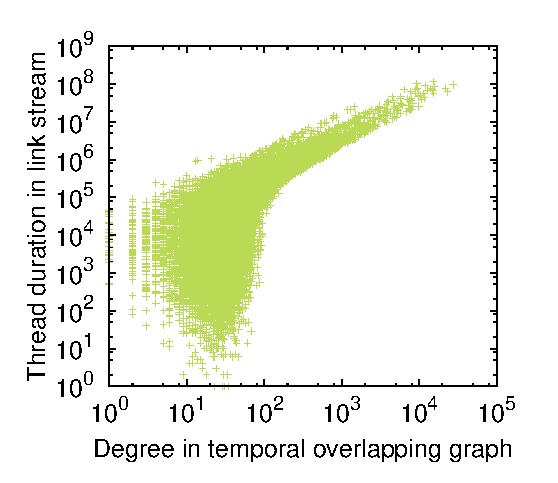
\includegraphics[width=0.49\linewidth]{img/mailing/degree_temp}
	\hfill
	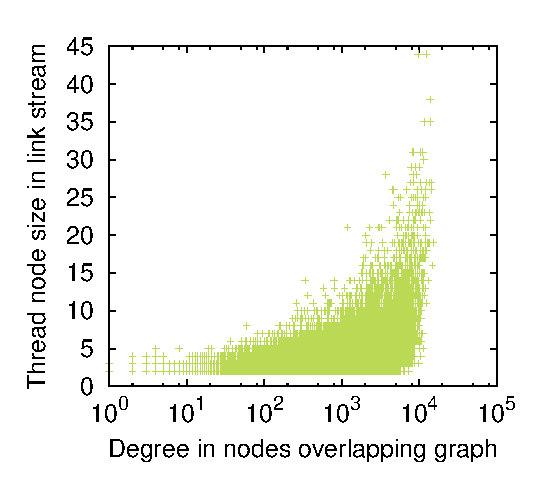
\includegraphics[width=0.49\linewidth]{img/mailing/degree_nodes}
	\caption{Gauche: Corrélation entre le degré des discussions dans le graphe de chevauchement temporel et leur durée. Droite: Corrélation entre le degré des discussions dans le graphe de chevauchement topologique et leur nombre de participants.}
	\label{fig:x-y-graphs_discu}
\end{figure}

La figure~\ref{fig:x-y-graphs_discu}(droite) présente la corrélation entre le degré d'une discussion dans le graphe de chevauchement topologique $Y$ et son nombre de participants.
La corrélation est moins nette mais il y a tout de même une tendance.



\section{Détection automatique des discussions?}

Nope